\begin{figure}
	\centering

	\hfill
	\subfloat[Original data flow graph]{\label{fig:innerSCCDataFlow}
	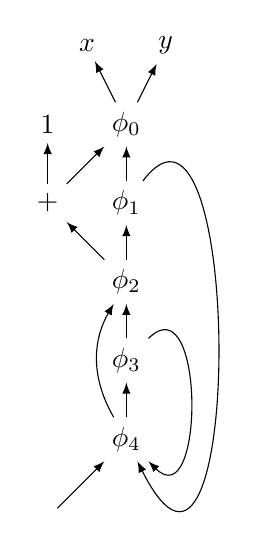
\begin{tikzpicture}
		\path
			  ( 0,   0) node (other)  {$\phi_0$}
			 +(-0.5, 1) node (x)      {$x$}
			 +( 0.5, 1) node (y)      {$y$}
			 +(-1,   0) node (one)    {$1$}
			++( 0,  -1) node (outer1) {$\phi_1$}
			++( 0,  -1) node (outer2) {$\phi_2$}
			 +(-1,   1) node (plus)   {$+$}
			++( 0,  -1) node (inner1) {$\phi_3$}
			++( 0,  -1) node (inner2) {$\phi_4$}
			 +(-1,  -1) node (use)    {}
		;
		\node at (1.2,0) {};
		\draw[-latex]         (other)  -> (x);
		\draw[-latex]         (other)  -> (y);
		\draw[-latex]         (plus)   -> (one);
		\draw[-latex]         (plus)   -> (other);
		\draw[-latex,overlay] (outer1) .. controls (1.5,1) and (1.5,-7) .. (inner2);
		\draw[-latex]         (outer1) -> (other);
		\draw[-latex]         (outer2) -> (outer1);
		\draw[-latex]         (outer2) -> (plus);
		\draw[-latex]         (inner1) -> (outer2);
		\draw[-latex,overlay] (inner1) .. controls (1,-2) and (1,-5) .. (inner2);
		\draw[-latex]         (inner2) edge[bend left] (outer2);
		\draw[-latex]         (inner2) -> (inner1);
		\draw[-latex]         (use)    -> (inner2);
	\end{tikzpicture}
	}
	\hfill
	\subfloat[SCCs and their operands]{\label{fig:innerSCCSCCs}
	\begin{tikzpicture}
		\path
			  ( 0,   0) node (other)  {$\phi_0$}
			 +(-0.5, 1) node (x)      {$x$}
			 +( 0.5, 1) node (y)      {$y$}
			++( 0,  -1) node (outer1) {$\phi_1$}
			++( 0,  -1) node (outer2) {$\phi_2$}
			 +(-1,   1) node (plus)   {$+$}
			++( 0,  -1) node (inner1) {$\phi_3$}
			++( 0,  -1) node (inner2) {$\phi_4$}
			 +(-1,  -1) node (use)    {}
		;
		\node at (1.2,0) {};
		\draw[-latex,dashed]  (other)  -> (x);
		\draw[-latex,dashed]  (other)  -> (y);
		\draw[-latex,overlay] (outer1) .. controls (1.5,1) and (1.5,-7) .. (inner2);
		\draw[-latex,dashed]  (outer1) -> (other);
		\draw[-latex]         (outer2) -> (outer1);
		\draw[-latex,dashed]  (outer2) -> (plus);
		\draw[-latex]         (inner1) -> (outer2);
		\draw[-latex,overlay] (inner1) .. controls (1,-2) and (1,-5) .. (inner2);
		\draw[-latex]         (inner2) edge[bend left] (outer2);
		\draw[-latex]         (inner2) -> (inner1);

		\begin{pgfonlayer}{background}
			\tikzselect{1}{
				(other.west) (other.north) (other.east) (other.south)
			}
			\tikzselect{0.3}{
				(outer1.west) (outer1.north) (outer1.east)
				(inner2.east) (inner2.south) (inner2.west)
			}
		\end{pgfonlayer}
	\end{tikzpicture}
	}
	\hfill
	\subfloat[Inner SCC]{\label{fig:innerSCCinnerSCC}
	\begin{tikzpicture}
		\path
			  (0, 0) node (outer1) {}
			++(0,-1) node (outer2) {$\phi_2$}
			++(0,-1) node (inner1) {$\phi_3$}
			++(0,-1) node (inner2) {$\phi_4$}
			 +(0,-1) node (use)    {}
		;
		\node at (0.8,0) {};
		\draw[-latex,overlay] (inner1) .. controls (1,-1) and (1,-4) .. (inner2);
		\draw[-latex,dashed]  (inner1) -> (outer2);
		\draw[-latex]         (inner2) -> (inner1);
		\draw[-latex,dashed]  (inner2) edge[bend left] (outer2);

		\begin{pgfonlayer}{background}
			\tikzselect{0.6}{
				(inner1.west) (inner1.north) (inner1.east)
				(inner2.east) (inner2.south) (inner2.west)
			}
		\end{pgfonlayer}
	\end{tikzpicture}
	}
	\hfill
	\subfloat[Optimized data flow graph]{\label{fig:innerSCCoptimized}
	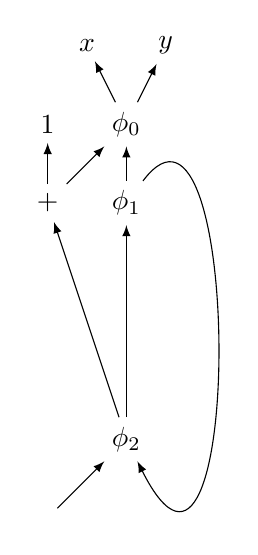
\begin{tikzpicture}
		\path
			  ( 0,   0) node (other)  {$\phi_0$}
			 +(-0.5, 1) node (x)      {$x$}
			 +( 0.5, 1) node (y)      {$y$}
			 +(-1,   0) node (one)    {$1$}
			++( 0,  -1) node (outer1) {$\phi_1$}
			 +(-1,   0) node (plus)   {$+$}
			++( 0,  -3) node (outer2) {$\phi_2$}
			 +(-1,  -1) node (use)    {}
		;
		\node at (1.2,0) {};
		\draw[-latex]         (other)  -> (x);
		\draw[-latex]         (other)  -> (y);
		\draw[-latex]         (plus)   -> (one);
		\draw[-latex]         (plus)   -> (other);
		\draw[-latex,overlay] (outer1) .. controls (1.5,1) and (1.5,-7) .. (outer2);
		\draw[-latex]         (outer1) -> (other);
		\draw[-latex]         (outer2) -> (outer1);
		\draw[-latex]         (outer2) -> (plus);
		\draw[-latex]         (use)    -> (outer2);
	\end{tikzpicture}
	}
	\hfill
	\caption{Some algorithm~\cite{braun13cc} detects the inner SCC spanned by $\phi_3$ and $\phi_4$. This SCC represents the same value. Thus, it gets replaced by $\phi_2$.}
\label{fig:optimizations}
\end{figure}
